\subsection{Architectural pattern}

Dự án sử dụng mô hình \textbf{MVCS}. Kiến trúc chuẩn của \textbf{MVCS} được thể hiện trong \ref{fig:mvcs-pattern}:

\begin{figure}[htbp]
    \centering
    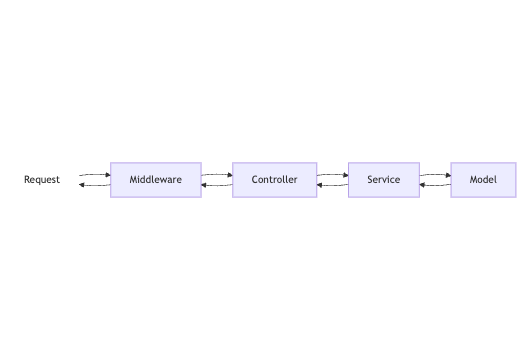
\includegraphics[width=0.8\textwidth]{Images/MVCS.png}
    \caption{MVCS pattern}
    \label{fig:mvcs-pattern}
\end{figure}

\textbf{MVCS} là viết tắt của \textbf{Model-View-Controller-Service}. Mô hình này cho phép lập trình viên định nghĩa trước sự tương tác giữa các phần code và dễ dàng chỉnh sửa bằng cách chia code thành các \textbf{layer} theo chức năng. Kiến trúc này không thuộc về bất kỳ ngôn ngữ lập trình hay framework cụ thể nào. \textbf{Pattern} này tách biệt \textbf{Database} hoặc \textbf{networking interaction} khỏi \textbf{Controller}. Mỗi phần đóng vai trò quan trọng trong việc phát triển ứng dụng.

\begin{itemize}
    \item \textbf{View Layer}: Đại diện cho cách dữ liệu được render lên giao diện người dùng. Trong dự án này, \textbf{View Layer} được xây dựng bằng \textbf{React.js} với các \textbf{Router} quản lý navigation và các \textbf{Component} hiển thị dữ liệu.
    \item \textbf{Controller Layer}: Chịu trách nhiệm chỉ nhận \textbf{request} và hiển thị kết quả của thao tác. \textbf{Controller} được sử dụng để giao tiếp giữa \textbf{Model}, \textbf{Service} và \textbf{View}. Trong \textbf{Backend Node.js}, các \textbf{Controller} như \textbf{Auth Controller}, \textbf{User Controller}, \textbf{Post Controller} xử lý các request từ \textbf{Frontend} và trả về \textbf{response} tương ứng.
    \item \textbf{Service Layer}: Còn được gọi là \textbf{Business Layer}, chứa các chức năng tạo nên core của ứng dụng, do đó trở nên \textbf{highly reusable} cho controllers và services. \textbf{Service Layer} xử lý \textbf{business logic} phức tạp, tách biệt khỏi \textbf{Controller} để dễ dàng maintain và test.
    \item \textbf{Model Layer}: Chịu trách nhiệm định nghĩa cách \textbf{data model} được định nghĩa. \textbf{Model Layer} sử dụng \textbf{Sequelize ORM} để ánh xạ các \textbf{entity} trong database như \textbf{User}, \textbf{Post}, \textbf{Product}, \textbf{Order}, \textbf{Message} và \textbf{Notification}.
\end{itemize}

\subsection{Architecture diagram}

\ref{fig:architecture-diagram} minh họa tổng quan cách chúng tôi lên kế hoạch triển khai hệ thống. Đối với \textbf{frontend}, tất cả các thiết kế đã được thực hiện với \textbf{Figma} sẽ được implement bằng \textbf{React.js} và cấu trúc được tổ chức như trong hình. \textbf{Frontend} được kết nối với \textbf{Backend Node.js} thông qua \textbf{HTTP request} và \textbf{WebSocket connection}.

\begin{figure}[htbp]
    \centering
    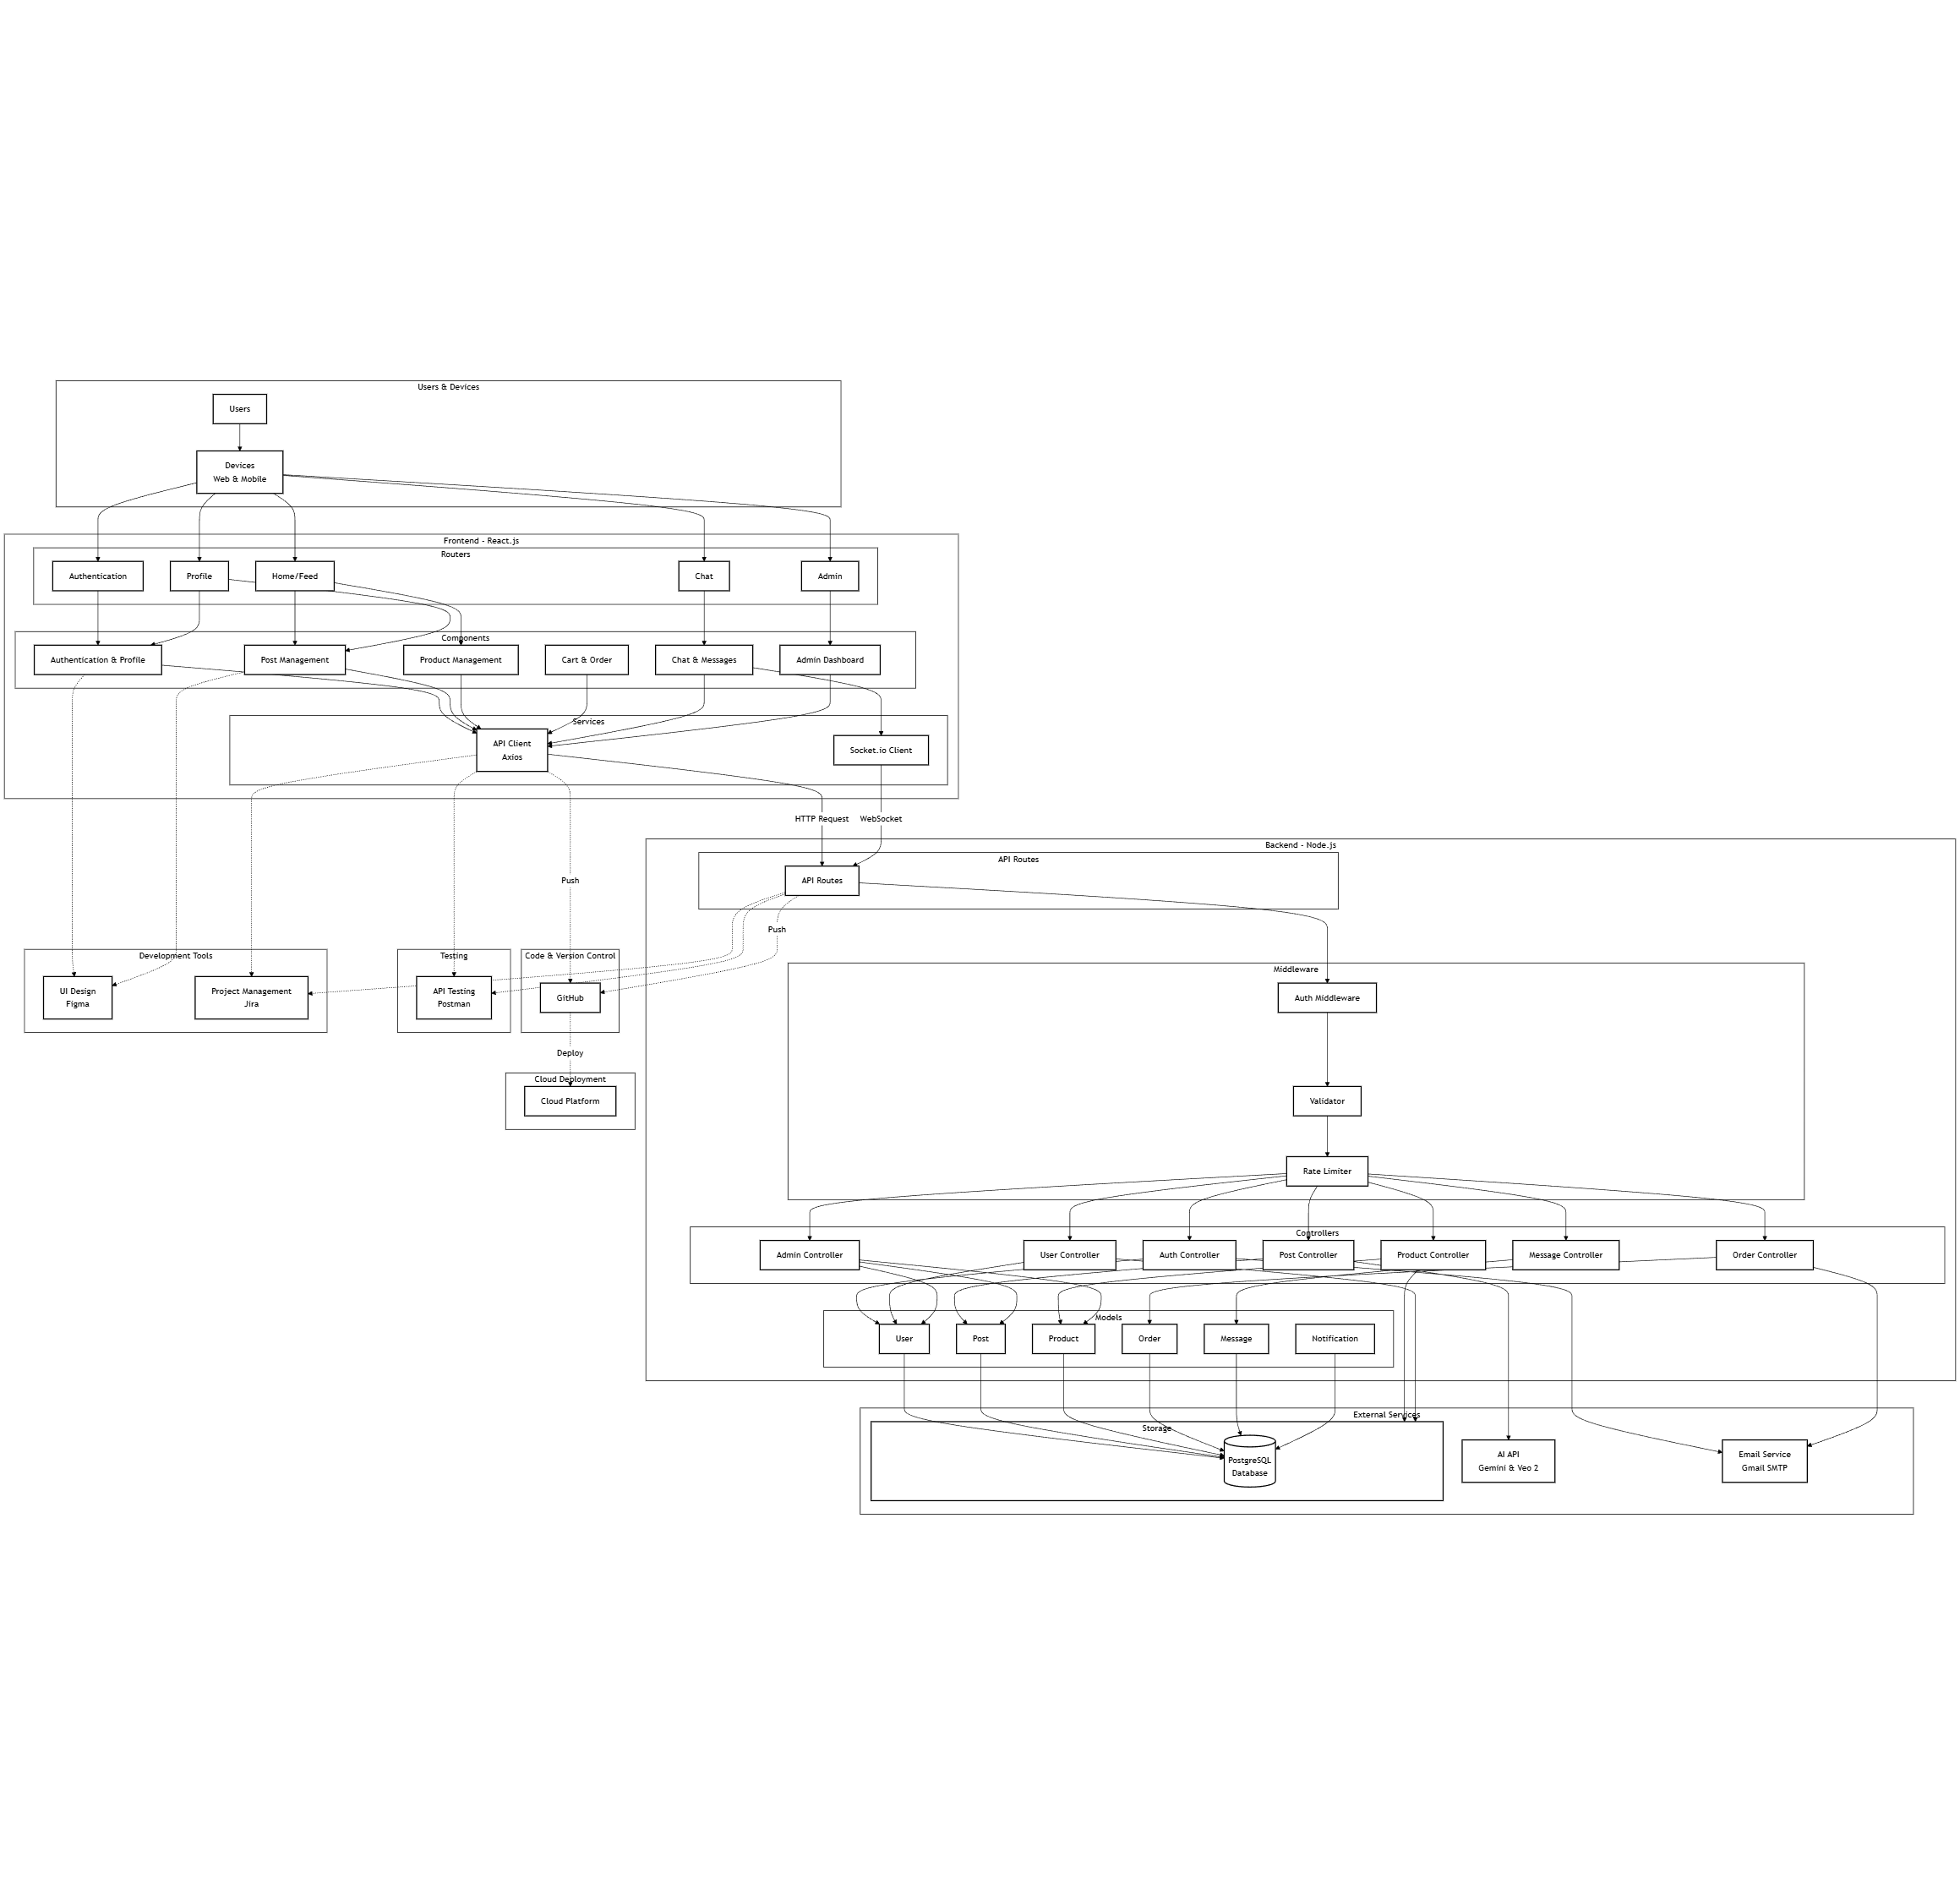
\includegraphics[width=1.0\textwidth]{Images/Architecture Diagram.png}
    \caption{Architecture Diagram for the system}
    \label{fig:architecture-diagram}
\end{figure}

\paragraph{Frontend Structure} Cấu trúc \textbf{Frontend} được tổ chức thành các thành phần chính:

\begin{itemize}
    \item \textbf{Routers}: Quản lý navigation giữa các trang
    \begin{itemize}
        \item \textbf{Authentication}: Trang xác thực người dùng
        \item \textbf{Home/Feed}: Trang chủ và bảng tin
        \item \textbf{Profile}: Trang hồ sơ người dùng
        \item \textbf{Chat}: Trang nhắn tin
        \item \textbf{Admin}: Trang quản trị
    \end{itemize}
    \item \textbf{Components}: Được tổ chức theo chức năng
    \begin{itemize}
        \item \textbf{Authentication \& Profile}: Xác thực và quản lý hồ sơ
        \item \textbf{Post Management}: Quản lý bài viết
        \item \textbf{Product Management}: Quản lý sản phẩm
        \item \textbf{Cart \& Order}: Giỏ hàng và đơn hàng
        \item \textbf{Chat \& Messages}: Tin nhắn và cuộc trò chuyện
        \item \textbf{Admin Dashboard}: Bảng điều khiển quản trị
    \end{itemize}
    \item \textbf{Services}: Kết nối với Backend
    \begin{itemize}
        \item \textbf{API Client (Axios)}: Thực hiện \textbf{HTTP request}
        \item \textbf{Socket.io Client}: Thiết lập kết nối \textbf{WebSocket} cho các tính năng \textbf{real-time}
    \end{itemize}
\end{itemize}

\paragraph{Backend Structure} \textbf{Backend} được xây dựng bằng \textbf{Node.js} với \textbf{Express.js framework}. Cấu trúc bao gồm:

\begin{itemize}
    \item \textbf{API Routes}: Đóng vai trò \textbf{entry point} nhận các request từ \textbf{Frontend}
    \item \textbf{Middleware}: Xử lý request qua chuỗi middleware
    \begin{itemize}
        \item \textbf{Auth Middleware}: Xác thực \textbf{JWT} và quản lý \textbf{session}
        \item \textbf{Validator}: Kiểm tra và validate dữ liệu đầu vào
        \item \textbf{Rate Limiter}: Giới hạn số lượng request để bảo vệ hệ thống
    \end{itemize}
    \item \textbf{Controllers}: Xử lý logic nghiệp vụ
    \begin{itemize}
        \item \textbf{Auth Controller}: Xử lý xác thực
        \item \textbf{User Controller}: Quản lý người dùng
        \item \textbf{Post Controller}: Quản lý bài viết
        \item \textbf{Product Controller}: Quản lý sản phẩm
        \item \textbf{Order Controller}: Quản lý đơn hàng
        \item \textbf{Message Controller}: Quản lý tin nhắn
        \item \textbf{Admin Controller}: Quản lý quản trị
    \end{itemize}
    \item \textbf{Models}: Đại diện cho các entity trong hệ thống
    \begin{itemize}
        \item \textbf{User}: Người dùng
        \item \textbf{Post}: Bài viết
        \item \textbf{Product}: Sản phẩm
        \item \textbf{Order}: Đơn hàng
        \item \textbf{Message}: Tin nhắn
        \item \textbf{Notification}: Thông báo
        \item Các Model hỗ trợ khác
    \end{itemize}
\end{itemize}

\paragraph{Database} Các \textbf{Model} này kết nối trực tiếp với database \textbf{PostgreSQL} thông qua \textbf{Sequelize ORM} để thực hiện các thao tác \textbf{CRUD} (Create, Read, Update, Delete).

\paragraph{Code \& Version Control} Để quản lý code và version, nhóm sử dụng \textbf{GitHub} và từ đó chúng tôi lên kế hoạch triển khai website thông qua \textbf{Cloud Platform} sử dụng các dịch vụ:

\begin{itemize}
    \item \textbf{Elastic Beanstalk}: Triển khai và quản lý ứng dụng
    \item \textbf{CodePipeline}: Tự động hóa quy trình CI/CD
    \item \textbf{Amazon RDS}: Quản lý database
\end{itemize}

Tất cả đều được cung cấp bởi các nhà cung cấp cloud.

\paragraph{Testing \& Development Tools} Hệ thống sử dụng các công cụ hỗ trợ:

\begin{itemize}
    \item \textbf{Testing}:
    \begin{itemize}
        \item \textbf{Postman}: Kiểm tra và đánh giá \textbf{API}
    \end{itemize}
    \item \textbf{Development Tools}:
    \begin{itemize}
        \item \textbf{Jira Software}: Bug tracking và project management
    \end{itemize}
\end{itemize}

\paragraph{External Services} Hệ thống tích hợp với các dịch vụ bên ngoài:

\begin{itemize}
    \item \textbf{AI API (Google Gemini \& Veo 2)}: Tạo nội dung đa phương thức (văn bản, hình ảnh, video ngắn)
    \item \textbf{File Storage (Cloudinary)}: Lưu trữ và quản lý hình ảnh
    \item \textbf{Email Service (Gmail SMTP)}: Gửi email xác thực và thông báo
\end{itemize}
